\documentclass[12pt]{beamer}
%\usetheme{Berkeley}
\usepackage[utf8]{inputenc}
\usepackage{amsmath}
\usepackage{amsfonts}
\usepackage{amssymb}
\usepackage{graphicx}
\usepackage{pifont}
\usepackage[absolute,overlay]{textpos}
\usepackage{todonotes}
%\author{}
%\title{}
%\setbeamercovered{transparent} 
%\setbeamertemplate{navigation symbols}{} 
%\logo{} 
%\institute{} 
%\date{} 
%\subject{} 

\setbeamercolor{frametitle}{fg=black}
\setbeamerfont{frametitle}{size=\huge,series=\bfseries}

\setbeamercolor{itemize item}{fg=black}
\setbeamercolor{itemize subitem}{fg=black}
\setbeamercolor{itemize subsubitem}{fg=black}
\setbeamertemplate{itemize item}{\normalsize\raise-1pt\hbox{\donotcoloroutermaths\ding{113}}}
\setbeamertemplate{itemize subitem}{\tiny\raise1.5pt\hbox{\donotcoloroutermaths$\blacksquare$}}
\setbeamertemplate{itemize subsubitem}{\footnotesize\raise1.5pt\hbox{\donotcoloroutermaths$\checkmark$}}

\usebackgroundtemplate{
\includegraphics[width=\paperwidth ,height=\paperheight]{media/template.pdf}
}

\beamertemplatenavigationsymbolsempty

\addtobeamertemplate{footline}{}{%
    \usebeamerfont{footline}%
    \usebeamercolor[fg]{footline}%
    \hspace{4.75in}%
    \vspace{.1in}
    \insertframenumber
}

\makeatletter
\setbeamertemplate{frametitle}{
    \ifbeamercolorempty[bg]{frametitle}{}{\nointerlineskip}%
    \@tempdima=\textwidth%
    \advance\@tempdima by\beamer@leftmargin%
    \advance\@tempdima by\beamer@rightmargin%
    \hspace*{1in} %%%%%%%%%%%%% For example insert shift to right
    \begin{beamercolorbox}[sep=.3cm,center,wd=\the\@tempdima]{frametitle}
        \usebeamerfont{frametitle}\Large%
        \vbox{}\vskip+.3in%
        \if@tempswa\else\csname beamer@ftecenter\endcsname\fi%
        \strut\insertframetitle\strut\par%
       
        {%
            \ifx\insertframesubtitle\@empty%
            \else%
            {\usebeamerfont{framesubtitle}\usebeamercolor[fg]{framesubtitle}\insertframesubtitle\strut\par}%
            \fi
        }%
        \vskip-1ex%
        \if@tempswa\else\vskip-.3cm\fi% set inside beamercolorbox... evil here...
    \end{beamercolorbox}%
}
\makeatother

\begin{document}

\begin{frame}
\begin{textblock}{20}(10,2)
\includegraphics[scale=.1]{media/logo.png}
\end{textblock}

\vspace{1in}
\huge Security of Distributed Cyber-Physical Systems (CPS) with Platoon Applications\\
\normalsize
\vspace{.25in}
\begin{center}
\large 
Dr. Richard Brooks \\
The Holcombe Department of Electrical and Computer Engineering\\
Clemson University
\end{center}
\end{frame}

\begin{frame}{Problem Statements}
\begin{itemize}
\item \textbf{Compromised subsystem in a distributed CPS}
\begin{itemize}
\item One or more than one subsystem are malicious and acting against a global goal.
\end{itemize}
\hfill 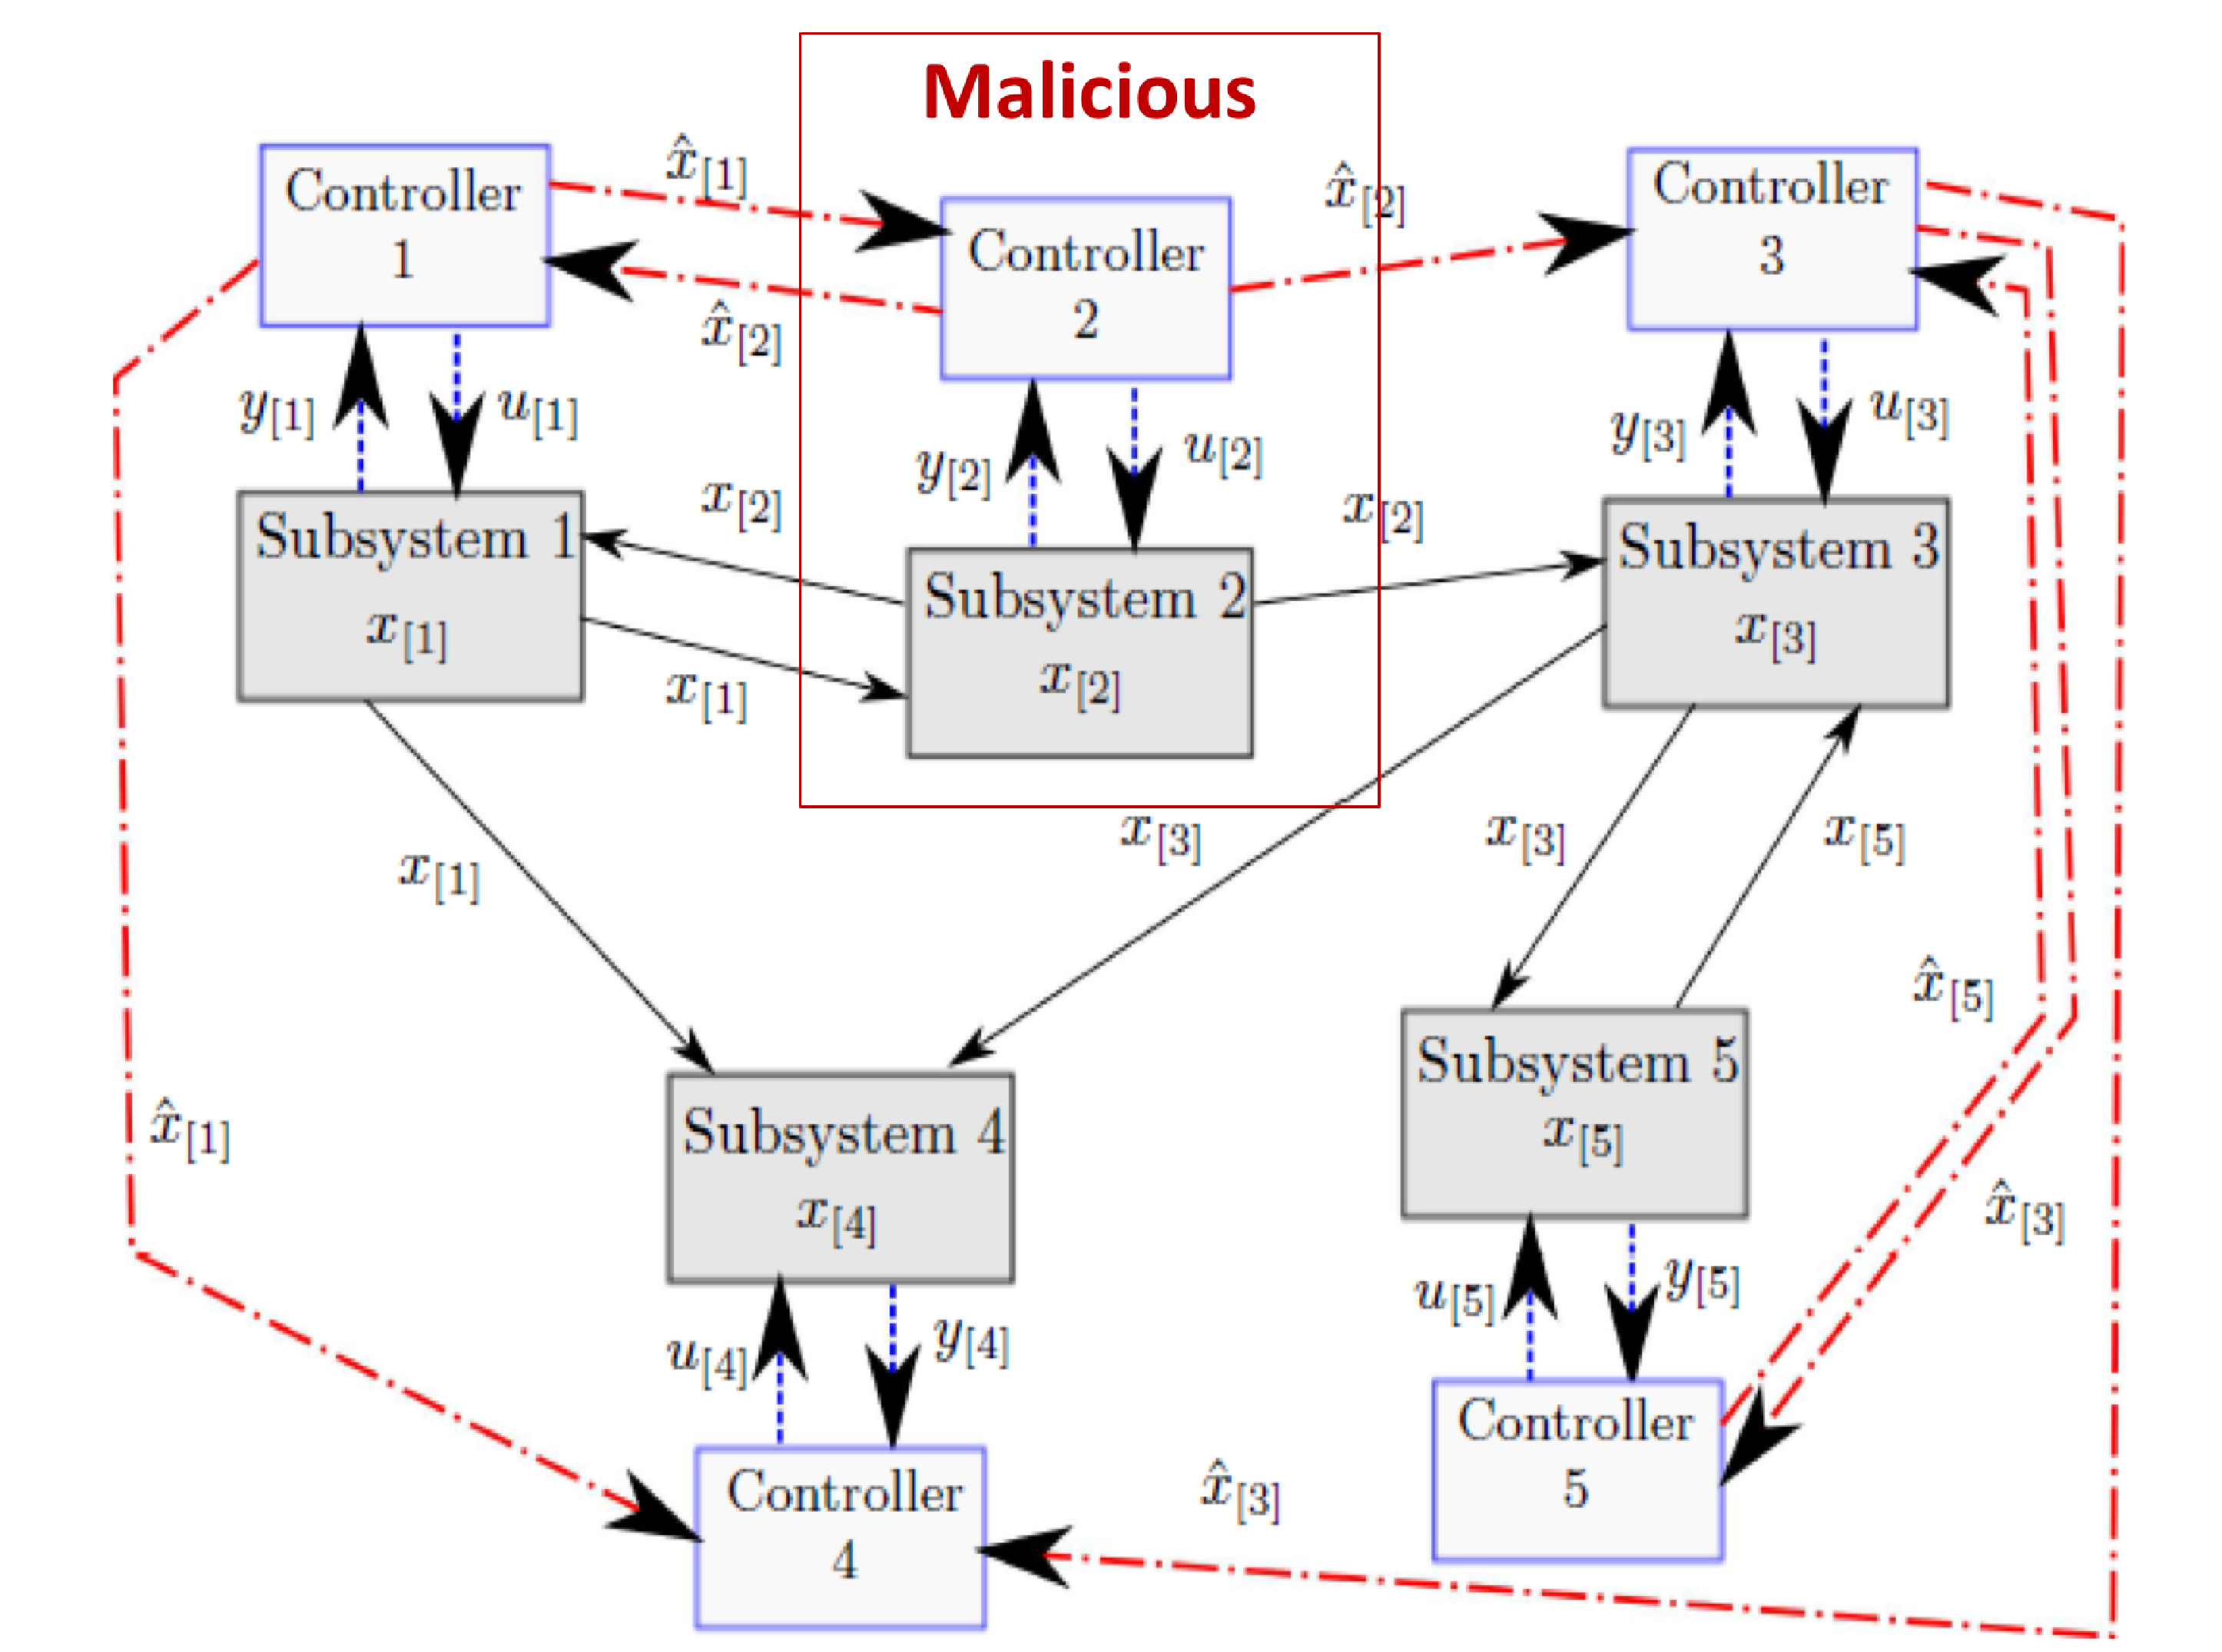
\includegraphics[scale=.1]{media/compromised.eps} \vspace{-.3in}
\item \textbf{Strategy}
\begin{itemize}
\item Game theory approach.
\item Design controller for rest of subsystems in the distributed CPS to keep the performance of the whole CPS close to normal.
\end{itemize}
\end{itemize}
\end{frame}

\begin{frame}{Platoon Models}
\begin{itemize}
\item \underline{\color{blue}Centralized  Control}: All vehicles send information to a centralized controller that makes the optimal decision to minimize total fuel consumption.


\item \underline{\color{blue}Decentralized Control}: Each vehicle makes its own decision based on local information to minimize its own fuel consumption.


\end{itemize}
\end{frame}

\begin{frame}{Controller Design}
\begin{itemize}
\item \textbf{Objective Function}:
\begin{align*} 
\tiny L_i(t) = \underbrace{w_1 \int_{\Delta t} \frac{\textrm{Fuel}}{v_i(t)}}_{\textrm{fuel consumption}}+ \underbrace{w_2 R_{\textrm{error}}^2 + w_6 R_{\textrm{error}'}^2}_{\textrm{distance}} + \underbrace{w_3(v_{i-1}(t+1) - v_{i}(t+1))^2}_{\textrm{$\Delta$v between car\textsubscript{i-1} and car\textsubscript{i}}} \\ \tiny
+ \underbrace{w_4a_i^2(t)}_{\textrm{acceleration}} +\underbrace{ w_5(v_{i+1}(t+1) - v_{i}(t+1))^2}_{\textrm{$\Delta$v between car\textsubscript{i} and car\textsubscript{i+1}}}
\end{align*}

\item Solve $\frac{\partial L_i(t)}{\partial a_i(t)} = 0$
\end{itemize}
\vspace{-.35in}
 \hfill \includegraphics[scale=.275]{media/acceleration.eps}

\end{frame}

\begin{frame}{Introducing Noise}

\end{frame}

\begin{frame}{Kalman Filter}

\end{frame}

\begin{frame}{?}

\end{frame}

%\begin{frame}{Previous Work}
%\begin{picture}(50,50)
%\put(200,10){\hbox{\includegraphics[scale=.05]{media/tor.png}}}
%\end{picture}
%\begin{picture}(50,50)
%\put(150,-50){\hbox{\includegraphics[scale=.2]{media/vpn.png}}}
%\end{picture}
%\vspace{-.5in}
%\begin{itemize}
%\item Tor
%\item VPN
%\item Decoy Routing
%\item Moving Target (NAT)
%\end{itemize}
%\end{frame}
%
%\begin{frame}{Hypothesis}
%\begin{columns}
%\begin{column}{0.5\textwidth}
%\begin{itemize}
%\item Hedy Lamarr
%\begin{itemize} \footnotesize
%\item Frequency Hop Spread Spectrum (FHSS)
%\end{itemize}
%\item \color{red}FHSS in IP address space
%\end{itemize}
%\end{column}
%\begin{column}{0.5\textwidth}  %%<--- here
%    \begin{center}
%     \includegraphics[scale=.5]{media/lamarr.jpg}
%     \end{center}
%\end{column}
%\end{columns}
%\end{frame}
%
%\begin{frame}{Hypothesis--Design}
%
%\end{frame}
%
%\begin{frame}{Future Work}
%\begin{itemize}
%\item Current Issues
%\begin{itemize}
%\item TSL leaks information.
%\item Choice of a session duration model.
%\item Bootstrapping synchronization of IP addresses.
%\end{itemize}
%\item Next Steps
%\begin{itemize}
%\item Implement two-way randomization.
%\item Implement SDX-based solution.
%\end{itemize}
%\end{itemize}
%\end{frame}

%\begin{frame}{}
%\begin{textblock}{20}(10,2)
%\includegraphics[scale=.1]{media/logo.png}
%\end{textblock}
%\vspace{.5in}
%\begin{center}\Large
%Contact
%\end{center}
%\begin{itemize}
%\item Xingsi Zhong, xingsiz@g.clemson.edu
%\item Lu Yu, lyu@g.clemson.edu
%\item Jon Oakley, joakley@g.clemson.edu
%\item Dr. Richard Brooks, rrb@g.clemson.edu
%\end{itemize}
%\end{frame}

%\begin{frame}{Background}
%\begin{itemize}
%\item test
%\begin{itemize}
%\item another
%\begin{itemize}
%\item item
%\end{itemize}
%\end{itemize}
%\end{itemize}
%\end{frame}

\end{document}